%!TeX spellcheck = en_US
\documentclass[12pt,a4paper,USenglish]{article}      % Specifies the document class
\usepackage[utf8]{inputenc}
\usepackage[T1]{fontenc,url}
\usepackage{babel,csquotes,newcent,textcomp}
\usepackage[backend=biber,sortcites]{biblatex}
\usepackage{graphicx}
%\usepackage{graphics}
%\usepackage{listings}

\usepackage{listings}
\usepackage{color}
\usepackage{comment}

\definecolor{dkgreen}{rgb}{0,0.6,0}
\definecolor{gray}{rgb}{0.5,0.5,0.5}
\definecolor{mauve}{rgb}{0.58,0,0.82}

\lstset{frame=tb,
  language=Java,
  aboveskip=3mm,
  belowskip=3mm,
  showstringspaces=false,
  columns=flexible,
  basicstyle={\small\ttfamily},
  numbers=left,
  numberstyle=\tiny\color{gray},
  keywordstyle=\color{blue},
  commentstyle=\color{dkgreen},
  stringstyle=\color{mauve},
  breaklines=true,
  breakatwhitespace=true,
  tabsize=3
}

\graphicspath{ {./images/} }

%\addbibresource{References.bib}

\title{Methodology}  % Declares the document's title.

%\newcommand{\ip}[2]{(#1, #2)}

\begin{document}             % End of preamble and beginning of text.
%\maketitle                   % Produces the title.
%\tableofcontents
\section{Cooperation test}
\subsection{Introduction}
The size of data that must be analyzed keeps increasing year after year and the prize for DRAM are not getting cheaper. NVDIMM offer a lot of storage at a cheaper prize. This opens the opportunity to save money by offloading some of the data to the NVDIMM where the data will be analyzed the same way as the data on the DRAM. The downside to this strategy is that NVDIMM is slower than DRAM so the question is how much data can be offloaded to NVDIMM. If the user offload too much data to NVDIMM then the threads working on analyzing the data on DRAM will be idle while waiting for NVDIMM threads to complete.

The goal of this benchmark is to find a formula that will make it possible to estimate how many threads should be delegated to work on the data located on NVDIMM. The methodology must also be able to calculate how much of the data on DRAM should be offloaded to NVDIMM

There is two version of the code that is being used. They have been programmed slightly different in the way read data. This is to explore which of them is the fastest.

%The goal is to find a formula that can easily calculate how much data can be offloaded to the NVDIMM from DRAM. The time taken to perform calculation on NVDIMM must be equal to the amount of time it takes to run calculation on the remaining data on DRAM. 

\subsection{Calculation of NVDIMM part}
\subsubsection{Formula}
In order to use the formula one must measure the NVDIMM and DRAM speed using a benchmark made in a previous chapter where speed was measured when data was transferred from DRAM to DRAM and from NVDIMM to NVDIMM simultaneously with different amount threads allocated to the different processes. By using using the speed from the benchmark in the formula below along with the size of the data that will be used in the calculation the user can easily calculate how much data can be transferred to NVDIMM without losing time. The formula does only decide how much data can be allocated to NVDIMM with a certain amount of threads. This means that the user must probably use the formula several times where the number of NVDIMM threads varies from one to five in order to find the best combination of threads and data allocated to the NVDIMM process. 
\\
\\
Formula
\begin{figure}
\[
    \frac{Total\_data-nvdimm\_data}{dram\_speed} = \frac{nvdimm\_data}{nvdimm\_speed}    
\]
\[
    nvdimm\_data = \frac{nvdimm\_speed*Total\_data}{nvdimm\_speed+dram\_speed}    
\]
\caption{The formula used to decide how much should be allocated to NVDIMM.}
\label{fig:mathFormula}
\end{figure}

I have created a benchmark that will test this formula to see if it is accurate.
This benchmark has an two dimensional array filled with data. The benchmark start at element (1,1) of the array where it sum ups all of its eight neighbors and then takes the average. The result is stored in the same position in another two dimensional array. The benchmark does this for every element between (1,1) and (m-2,n-2). 
The benchmark repeats this process ten times and after each time the benchmark will swap both the DRAM arrays and NVDIMM array. The time is measured at the beginning of the process and at the end, this time is called total\_time in the code.
Each thread will also measure the time they takes to complete their own tasks, in the code this is called individual\_time.

In listing \ref{lst:LABserial} is an example of the serial code of the benchmark. The array has not been divided into two.
The thread will will repeat the while-loop on line 1 k\_length amount of time. It will start the time measurement at line 2. From line 3-10 the thread will pass through the the 2D-array row by row starting from element (1,1) and end at element (m-2,n-2). At each element the thread will calculate the average of all the elements neighbors, eight neighbors in total.
The thread will then stop the time measurement at line 11 and swap the arrays at line 12-14.
It will also increase k by one and start over if k is still lower than k\_length.

\begin{lstlisting}[caption={Serial code of the code that will be used in the first and second version.}, label={lst:LABserial}]
while(k<K_length){
	total_time[k] = mysecond();
	for( i=1; i<m-2; i++){
		for( j=1; j<n-2; j++){
			temp =  A[i-1][j-1] + A[i-1][j] + A[i-1][j+1]+
					    A[i][j-1]        +        A[i][j+1]+
					    A[i+1][j-1] + A[i+1][j] + A[i+1][j+1];
			B[i][j] = temp/8;
		}
	}
	total_time[k] = mysecond() - total_time[k];
	temp_array = A;
	A = B;
	B = temp_array;
	k++;
}
\end{lstlisting}

\begin{comment}
Table 1 shows the calculation of how much data must be allocated to NVDIMM in order for the DRAM and NVDIMM to complete their tasks simultaneously. M in row one in table shows how many rows the 2D-array has. The n in row two shows how many elements each row has. The total MB in row three is calculated in following manner, m*n/(8*1000000). Row five is the beginning of five column. First column shows how many threads are used to calculate data on NVDIMM. Second and third column is the DRAM and NVDIMM speed in MB per second. The speeds comes from a benchmark described in a previous chapter where data is transferred from DRAM-DRAM and NVDIMM-NVDIMM simultaneously. Column four uses the formula described in the beginning of the chapter, the numbers are in MB. The last column converts the result in fourth column into number of rows of the 2D-array that will be placed on NVDIMM.
\begin{table}[!hbtp]
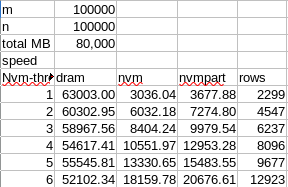
\includegraphics[scale=0.6]{Large_Array_test/First_version_100k_100k_Distibution_v2.png}
\caption{First version, distribution}
\end{table}
\end{comment}

\subsubsection{Distribution}
By using the formula described above we have calculated the distribution of data between DRAM and NVDIMM in table \ref{tab:distribution16GB} and \ref{tab:distribution160GB}. The tables show the number of NVDIMM threads assigned in first column. Second and third column shows the speed of DRAM and NVDIMM. The speed is from the result of the benchmark in section x.x. Fourth column shows how much data should be placed on NVDIMM. This is based on the formula described previously in this chapter. The last column shows how many rows in the 2D array of data must be delegated to NVDIMM in order for the size of the array to be equal to the previous column.

\begin{table}[!hbtp]
\centering
\begin{tabular}{ |c|c|c|c|c| } 
\hline
Threads & DRAM & NVDIMM & NVDIMM part & NVDIMM rows \\
\hline
1 & 61042.84 & 3038.16 & 379.30 & 750 \\
\hline
2 & 57761.80 & 6027.24 & 755.91 & 1494 \\
\hline
3 & 53767.10 & 9223.43 & 1171.42 & 2315 \\
\hline
4 & 51257.79 & 12630.42 & 1581.59 & 3126 \\
\hline
5 & 47770.89 & 15202.48 & 1931.32 & 3817 \\
\hline
\end{tabular}
\caption{Distribution of 16 GB data between DRAM and NVDIMM.}
\label{tab:distribution16GB}
\end{table}

\begin{table}[!hbtp]
\centering
\begin{tabular}{ |c|c|c|c|c| } 
\hline
Threads & DRAM & NVDIMM & NVDIMM part & NVDIMM rows \\
\hline
1 & 61042.84 & 3038.16 & 3792.90 & 2371 \\
\hline
2 & 57761.80 & 6027.24 & 7558.96 & 4724 \\
\hline
3 & 53767.10 & 9223.43 & 11714.05 & 7321 \\
\hline
4 & 51257.79 & 12630.42 & 15815.65 & 9885 \\
\hline
5 & 47770.89 & 15202.48 & 19312.90 & 12071 \\
\hline
\end{tabular}
\caption{Distribution of 160 GB data between DRAM and NVDIMM.}
\label{tab:distribution160GB}
\end{table}

%Distribution of m\\
%\subsection{Prediction}
\subsubsection{Prediction}
The distributions calculated in the previous section are used in this section to predict how much time DRAM and NVDIMM will take to complete their tasks.
The first column the number NVDIMM threads. Second and fifth column shows the speed of DRAM and NVDIMM, they are also from the result of the benchmark in section x.x.
Third and sixth column shows how much data is allocated to DRAM and NVDIMM. Fourth and seventh column shows the how much time it takes for DRAM and NVDIMM to complete their tasks.

\begin{table}[!hbtp]
\begin{tabular}{ |c|c|c|c|c|c|c| }
\hline
        & DRAM  & DRAM & DRAM      & NVDIMM & NVDIMM & NVDIMM \\
Threads & speed & Size & pred.time & speed  & Size   & pred.time \\
\hline
1 & 61042.84 & 15241.41 & 0.2497 & 3038.16 & 758.59 & 0.2497 \\
\hline
2 & 57761.80 & 14488.19 & 0.2508 & 6027.24 & 1511.81 & 0.2508 \\
\hline
3 & 53767.10 & 13657.16 & 0.2540 & 9223.43 & 2342.84 & 0.2540 \\
\hline
4 & 51257.79 & 12836.82 & 0.2504 & 12630.42 & 3163.18 & 0.2504 \\
\hline
5 & 47770.89 & 12137.37 & 0.2541 & 15202.48 & 3862.63 & 0.2541 \\
\hline
\end{tabular}
\caption{Time prediction with 16 GB of data.}
\label{tab:Prediction16GB}
\end{table}

\begin{table}[!hbtp]
\begin{tabular}{ |c|c|c|c|c|c|c| }
\hline
        & DRAM  & DRAM & DRAM      & NVDIMM & NVDIMM & NVDIMM \\
Threads & speed & Size & pred.time & speed  & Size   & pred.time \\
\hline
1 & 61042.84 & 152414.20 & 3.7453 & 3038.16 & 7585.80 & 3.7453 \\
\hline
2 & 57761.80 & 144882.07 & 3.7624 & 6027.24 & 15117.93 & 3.7624 \\
\hline
3 & 53767.10 & 136571.90 & 3.8101 & 9223.43 & 23428.10 & 3.8101 \\
\hline
4 & 51257.79 & 128368.69 & 3.7566 & 12630.42 & 31631.31 & 3.7566 \\
\hline
5 & 47770.89 & 121374.21 & 3.8111 & 15202.48 & 38625.79 & 3.8111 \\
\hline
\end{tabular}
\caption{Time prediction with 160 GB of data.}
\label{tab:Prediction160GB}
\end{table}

\begin{comment}
\begin{table}[!hbtp]
\centering
\begin{tabular}{ |c|c|c|c|c|c|c| } 
\hline
        & DRAM  & DRAM & DRAM      & NVDIMM & NVDIMM & NVDIMM \\
Threads & speed & Size & pred.time & speed  & Size   & pred.time \\
\hline
1 & 61042.84 & 15620.75 & 0.2559 & 3038.16 & 379.48 & 0.1249 \\
\hline
2 & 57761.80 & 15244.31 & 0.2639 & 6027.24 & 755.92 & 0.1254 \\
\hline
3 & 53767.10 & 14828.91 & 0.2758 & 9223.43 & 1171.32 & 0.1270 \\
\hline
4 & 51257.79 & 14418.57 & 0.2813 & 12630.42 & 1581.66 & 0.1252 \\
\hline
5 & 47770.89 & 14068.95 & 0.2945 & 15202.48 & 1931.28 & 0.1270 \\
\hline
\end{tabular}
\caption{Prediction, 16 GB}
\label{tab:Prediction16GB}
\end{table}
\begin{table}[!hbtp]
\centering
\begin{tabular}{ |c|c|c|c|c|c|c| }
\hline
 & DRAM & DRAM & DRAM & NVDIMM & NVDIMM & NVDIMM \\
Threads & speed & Size & pred.time & speed & Size & pred.time \\
\hline
1 & 61042.84 & 156206.40 & 3.8384 & 3038.16 & 3793.60 & 1.8730 \\
\hline
2 & 57761.80 & 152441.60 & 3.9587 & 6027.24 & 7558.40 & 1.8811 \\
\hline
3 & 53767.10 & 148286.40 & 4.1369 & 9223.43 & 11713.60 & 1.9050 \\
\hline
4 & 51257.79 & 144184.00 & 4.2194 & 12630.42 & 15816.00 & 1.8783 \\
\hline
5 & 47770.89 & 140686.40 & 4.4175 & 15202.48 & 19313.60 & 1.9056 \\
\hline
\end{tabular}
\caption{Prediction, 160 GB}
\label{tab:Prediction160GB}
\end{table}
\end{comment}

\subsection{First version}
There are two groups of threads that works in parallel in this program. The first group of threads works on the part of the data that is stored on DRAM and the other works on the data stored on NVDIMM. 
One thread in each group works on data that borders with the other group. In the DRAM group that is the thread with the highest thread\_id. Each of the elements in the last row of data will have three neighbors that exist on the NVDIMM side. This means that the thread must access the NVDIMM in order to get the data. The NVDIMM thread with the lowest thread\_id also have elements in the first row of data that have three neighbours that exist in DRAM that must be accessed by the thread directly.
%\\
%\\
%Explaination of code:\\

The code below only shows the calculation process, it does not the rest of the code. Allocation of memory have been done by all the threads, as a result the data have been spread across all the memory channels. 
The data is a 2d array where the rows of data on DRAM will be divided equally between the DRAM threads, the rows of data on NVDIMM will also be divided equally between the NVDIMM threads. The variable slice\_start hold the index of the row where the tread must start at and slice\_end holds the index of the row the thread must stop at.
Array A and B are DRAM array and array C and D are NVDIMM arrays. The average found by adding together eight neighbors in A will be placed in same position in B. The same is true for C and D.

The process are repeated K\_length amount of time, usually ten times in my tests. One way of knowing if the test result are correct is to run the test several time and look for consistency.
The code measures the time taken to complete one iteration of calculation, this is done in the beginning of the code at line 5 and at the end at line 84 by a single thread.
All the threads then get divided into the DRAM and NVDIMM at line 8. If the thread\_id of a thread is less than the dram\_threads is it will do calculation on the data in DRAM, the rest will fail the if test and move on to the else bracket at line 42. Dram\_threads is the total amount of threads that will be working on data in DRAM.

At line 11 the thread with the highest thread\_id will pass the if test and the rest will move on to line 30. The thread with highest thread\_id will then measure time at line 12 and end the measurement in line 29, this is the start and the end of the bracket. The thread will then enter a double for-loop at line 13-20 that will go through elements from position (slice\_start,1) until (slice\_end-1,n-1), this leaves out the last row assigned to the tread, that row will be dealt with later. At each element the for-loop it will add all of its eight neighbors together at line 15-17 and divide by eight at line 18.
The thread will then enter a new for-loop at line 23, this for-loop will calculate average of the last row on DRAM. Elements of this row have three neighbors that exist in NVDIMM. The thread will access the NVDIMM directly when adding the eight neighbors at line 24-26. Data on NVDIMM are accessed by the thread at line 26, the thread is using a library developed for this purpose. 

For all the other DRAM threads that jumped to line 30 will start by taking time measurement at the beginning and at the end of the bracket at line 31 and 40. The code from line 32-39 is identical to line 13-20 describe before.

The group of NVDIMM enters the else bracket at line 42 where the thread with the lowest thread\_id will pass the if-sentence at line 44, the rest will move on to the else bracket at line 62. The thread will then measure time at line 45 and end the measurement in line 61.
It will then enter a for-loop at line 47 and will begin calculating the average of the neighbors of the elements in the first row. The first row have three of its eight neighbors in the row above and they exist in the DRAM.
Once done the thread will move on to a new for-loop at line 53. This for-loop will go through the rest of the portion of data the thread have been given and calculate the average of each elements neighbors.

The rest of the NVDIMM threads will move into the else bracket at line 62. The code here is very similar to the code at 31-40 that has been described at a previous paragraph. The only difference is that the code at line 66-68 where the code reads from NVDIMM instead DRAM.

All the threads will wait a barrier at line 75 until all threads are done. After that on thread will enter a single bracket where array A and B will swap places, array C and D will also swap places. The time it took for this one iteration will be registered at line 84. After this the code will move back to line 1.


\begin{lstlisting}[caption=First version of the code where the threads will access data on the other memory type directly.]
while(k<K_length){
	#pragma omp barrier
	#pragma omp single
	{
		total_time[k] = mysecond();
	}
	//Divides threads into DRAM threads and NVDIMM threads.
	if( thread_id < dram_threads ){

		//for the thread bordering on NVDIMM thread.
		if( thread_id==(dram_threads-1) ){
			individual_time[k][thread_id] = mysecond();
			for( i=slice_start; i<slice_end-1; i++){
				for( j=1; j<nMinusOne; j++){
					temp = A[i-1][j-1] + A[i-1][j] + A[i-1][j+1]+
						   A[i][j-1]        +        A[i][j+1]+
					       A[i+1][j-1] + A[i+1][j] + A[i+1][j+1];
					B[i][j] = temp*inverseEigth;
				}
			}
			
			i = slice_end-1;
			for( j=1; j<nMinusOne; j++){
				temp = A[i-1][j-1] + A[i-1][j] + A[i-1][j+1]+
					    A[i][j-1]        +        A[i][j+1]+
				       D_RO(C)[i*n+j] + D_RO(C)[i*n+j] + D_RO(C)[i*n+j];
				B[i][j] = temp*inverseEigth;
      		}
			individual_time[k][thread_id] = mysecond() - individual_time[k][thread_id];
		}else{
			individual_time[k][thread_id] = mysecond();
			for( i=slice_start; i<slice_end; i++){
				for( j=1; j<nMinusOne; j++){
					temp = A[i-1][j-1] + A[i-1][j] + A[i-1][j+1]+
						   A[i][j-1]        +        A[i][j+1]+
						   A[i+1][j-1] + A[i+1][j] + A[i+1][j+1];
					B[i][j] = temp*inverseEigth;
				}
			}
			individual_time[k][thread_id] = mysecond() - individual_time[k][thread_id];
		}
	}else{
		//for the thread bordering on DRAM thread.
		if( thread_id==dram_threads ){
			individual_time[k][thread_id] = mysecond();
			i=0;
			for( j=1; j<nMinusOne; j++){
				temp = A[dram_part-1][j-1]+A[dram_part-1][j]+A[dram_part-1][j+1]+
					   D_RO(C)[i*n+(j-1)]            +            D_RO(C)[i*n+(j+1)]+
					   D_RO(C)[(i+1)*n+(j-1)] + D_RO(C)[(i+1)*n+j] + D_RO(C)[(i+1)*n+(j+1)];
				D_RW(D)[i*n+j] = temp*inverseEigth;
			}
			for( i=slice_start+1; i<slice_end-1; i++){
				for( j=1; j<nMinusOne; j++){
					temp = D_RO(C)[(i-1)*n+(j-1)] + D_RO(C)[(i-1)*n+j] + D_RO(C)[(i-1)*n+(j+1)]+
						   D_RO(C)[i*n+(j-1)]            +            D_RO(C)[i*n+(j+1)]+
						   D_RO(C)[(i+1)*n+(j+1)] + D_RO(C)[(i+1)*n+j] + D_RO(C)[(i+1)*n+(j+1)];
					D_RW(D)[i*n+j] = temp*inverseEigth;
				}
			}
			individual_time[k][thread_id] = mysecond() - individual_time[k][thread_id];
		}else{
			individual_time[k][thread_id] = mysecond();
			for( i=slice_start; i<slice_end; i++){
				for( j=1; j<nMinusOne; j++){
					temp = D_RO(C)[(i-1)*n+(j-1)] + D_RO(C)[(i-1)*n+j] + D_RO(C)[(i-1)*n+(j+1)]+
						   D_RO(C)[i*n+(j-1)]            +            D_RO(C)[i*n+(j+1)]+
						   D_RO(C)[(i+1)*n+(j-1)] + D_RO(C)[(i+1)*n+j] + D_RO(C)[(i+1)*n+(j+1)];
                    D_RW(D)[i*n+j] = temp*inverseEigth;
				}
			}
			individual_time[k][thread_id] = mysecond() - individual_time[k][thread_id];
		}
	}
	#pragma omp barrier
	#pragma omp single
	{
		tempArray = B;
        B=A;
        A=tempArray;
		temp_nvdimm = C;
		C = D;
		D = temp_nvdimm;
		total_time[k] = mysecond() - total_time[k];
		k++;
	}
	#pragma omp barrier
}//End of while
\end{lstlisting}


In table two the first two column shows m and n. Third column shows how many rows are assigned to NVDIMM. Fourth and fifth column shows the number of DRAM and NVDIMM threads the test have used.
Column five and six shows the time it takes for DRAM and NVDIMM to complete their tasks. Column seven show the total time for the test.

Each row in table \ref{tab:FirstVersion16GB} and \ref{tab:FirstVersion160GB} are the result of running the code shown above one time. The code run its test ten times and all threads measures the time it takes to complete their own tasks. The slowest DRAM thread and slowest NVDIMM thread in each test gets stored. The time shown in column six and seven is the average of those times. Total time in column eight is the average time it takes for all the threads to complete.

\begin{table}[!hbtp]
\begin{tabular}{ |c|c|c|c|c|c|c|c| }
\hline
&  & NVDIMM & DRAM & NVDIMM & DRAM & NVDIMM & Total \\
M & N & rows & threads & threads & time & time & time \\
\hline
31623 & 31623 & 750 & 15 & 1 & 0.3099 & 0.3431 & 0.3457 \\
\hline
31623 & 31623 & 1494 & 14 & 2 & 0.3117 & 0.3416 & 0.3427 \\
\hline
31623 & 31623 & 2315 & 13 & 3 & 0.2937 & 0.3522 & 0.3542 \\
\hline
31623 & 31623 & 3126 & 12 & 4 & 0.2882 & 0.3571 & 0.3578 \\
\hline
31623 & 31623 & 3817 & 11 & 5 & 0.2900 & 0.3510 & 0.3512 \\
\hline
\end{tabular}
\caption{Result of the first version of the code with 16 GB of data.}
\label{tab:FirstVersion16GB}
\end{table}
\begin{figure}[!hbtp]
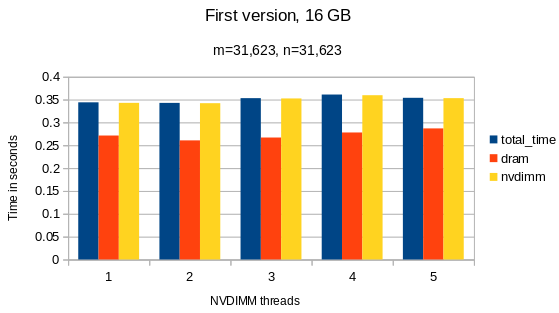
\includegraphics[scale=0.7]{Large_Array_test/First_version_16GB.png}
\caption{Result of the first version of the code with 16 GB of data in graph form.}
\label{fig:FirstVersion16GB}
\end{figure}

The DRAM times of the in table \ref{tab:FirstVersion16GB} are almost matching the predicted times in table \ref{tab:Prediction16GB}. The difference between predicted time and actual time is at most 0.05 seconds.
When comparing the predicted DRAM time in table \ref{tab:Prediction160GB} and actual DRAM time in table \ref{tab:FirstVersion160GB} one can see that predicted time is very close to actual time. The biggest difference is when there are four NVDIMM threads. With four NVDIMM threads the difference is 0.24 seconds.

The NVDIMM time predictions are a lot worse. According to the prediction the DRAM and NVDIMM are supposed to complete at the same time, but this is not happening. When comparing the predicted time for NVDIMM in table \ref{tab:FirstVersion16GB} with the measured time in table \ref{tab:Prediction16GB} one can see that NVDIMM a lot longer time to complete. NVDIMM use about 0.1 second longer to complete its tasks, this is about 30\% longer than predicted time.
The difference becomes even greater when the size of the array increases. The NVDIMM predicted time in table \ref{tab:Prediction160GB} is in the range of between 3.74 and 3,81 seconds depending on how many threads are given to NVDIMM. The time it takes for NVDIMM to complete their task is almost twice as long for all the tests.

Since the time prediction for the DRAM was accurate this should mean that there isn't anything wrong with the prediction. The NVDIMM have performed slower than expected based on the benchmarks collected in section \ref{section:NVM-NVM}.

The total time in table \ref{tab:FirstVersion16GB} is almost identical to the NVDIMM. This makes sense because the only thing happening the threads are not doing their tests is the swapping of arrays and this takes almost no time at all. Since the slowest thread is always an NVDIMM then the total time should be equal to the NVDIMM time.

This is not the case however in the table \ref{tab:FirstVersion160GB}. Total time in this result is only once identical to the NVDIMM time and that is when NVDIMM is given five threads. For all the other total times there are a time difference of between 0,5 and 2 seconds. 
Based on the code the total time should be identical to NVDIMM time like the result in table \ref{tab:FirstVersion16GB} was. The only difference between these results are that the arrays are bigger, but that should not affect the time it take to swap arrays. 

\begin{table}[!hbtp]
\centering
\begin{tabular}{ |c|c|c|c|c|c|c|c| }
\hline
&  & NVDIMM & DRAM & NVDIMM & DRAM & NVDIMM & Total \\
M & N & rows & threads & threads & time & time & time \\
\hline
100000 & 100000 & 2371 & 15 & 1 & 3.7423 & 4.4166 & 6.1124 \\
\hline
100000 & 100000 & 4724 & 14 & 2 & 4.0061 & 5.0799 & 7.1181 \\
\hline
100000 & 100000 & 7321 & 13 & 3 & 4.0294 & 7.3525 & 7.8412 \\
\hline
100000 & 100000 & 9885 & 12 & 4 & 4.0449 & 6.2484 & 7.3231 \\
\hline
100000 & 100000 & 12071 & 11 & 5 & 4.0556 & 7.7680 & 7.7681 \\
\hline
\end{tabular}
\caption{Result of the first version of the code with 16 GB of data.}
\label{tab:FirstVersion160GB}
\end{table}
\begin{figure}[!hbtp]
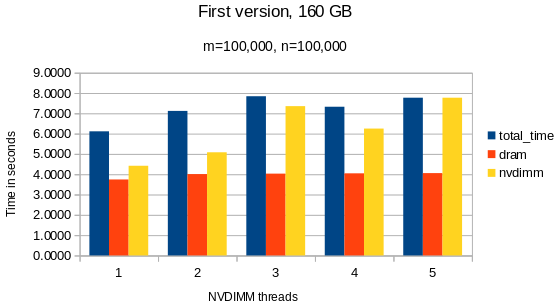
\includegraphics[scale=0.7]{Large_Array_test/First_version_160GB.png}
\caption{Result of the first version of the code with 16 GB of data in graph form.}
\label{fig:FirstVersion160GB}
\end{figure}

\clearpage
\subsection{Second version}
Same as the first version there are two groups of threads that works in parallel in this program. The first group of threads works on the part of the data that is stored on DRAM and the other works on the data stored on NVDIMM.
In this version the two threads that has a row of elements with neighbours in the other type of memory will not directly access this data. Instead the two arrays will have their own ghost array on their memory that they will access instead of fetching data from the other side. 

The while loop in line 1 will repeat itself for K\_length amount of time usually ten times, this is decided by the user of the benchmark. All the threads will wait for all the other threads to arrive at line 2 before one of the threads will start the time measurement in line 5.
When the threads arrives at line 8 the all the DRAM threads will pass the if-test and all the NVDIMM threads will move on to line 19. The DRAM threads will first start the time measurement in line 9 and will then start to calculate the average for every elements in the  part of the array that have been allocated to the each of the threads, this will happen from line 10-17. The threads will then stop the time measurement in line 18.

The NVDIMM threads will enter the else bracket at line 19. The threads will then start time measurement at line 20. From line 21-28 the threads will calculate average on the elements that have been assigned to each thread. At line 29 the threads will stop the time measurements.

The DRAM and NVDIMM threads will then encounter a barrier at line 31 where they will wait for all the other threads to finish. All threads will then update the ghost arrays at line 34 and 35. At line 34 the threads are copying the second row in the NVDIMM array into the last row in the DRAM array. In line 35 they are copying the second last row in the DRAM array into the first row in the NVDIMM array.

Once all the threads are done copying their parts of the rows, one thread will enter the single at line 37. This thread will swap the DRAM arrays and then the NVDIMM array. The thread will then stop the time measurement that was at the beginning of the while-loop at line 47. At line 48 the k variable gets increased by one. The threads will then return to line 1. 

\begin{lstlisting}[caption=Second version of the code where the threads are using ghost array instead of accessing the other type of memory directly.]
while(k<K_length){
	#pragma omp barrier
	#pragma omp single
	{
		total_time[k] = mysecond();
	}
	//Divides threads into DRAM threads and NVDIMM threads.
	if( thread_id < dram_threads ){
		individual_time[k][thread_id] = mysecond();
		for( i=slice_start; i<slice_end; i++){
			for( j=1; j<nMinusOne; j++){
				temp = A[i-1][j-1] + A[i-1][j] + A[i-1][j+1]+
						A[i][j-1]       +       A[i][j+1]+
						A[i+1][j-1] + A[i+1][j] + A[i+1][j+1];
				B[i][j] = temp*inverseEigth;
			}
		}
		individual_time[k][thread_id] = mysecond() - individual_time[k][thread_id];
	}else{
	individual_time[k][thread_id] = mysecond();
		for( i=slice_start; i<slice_end; i++){
        	for( j=1; j<nMinusOne; j++){
        		temp = D_RO(C)[(i-1)*n+(j-1)] + D_RO(C)[(i-1)*n+j] + D_RO(C)[(i-1)*n+(j+1)]+
        				D_RO(C)[i*n+(j-1)]            +            D_RO(C)[i*n+(j+1)]+
        				D_RO(C)[(i+1)*n+(j-1)] + D_RO(C)[(i+1)*n+j] + D_RO(C)[(i+1)*n+(j+1)];
        		D_RW(D)[i*n+j] = temp*inverseEigth;
        	}
        }
		individual_time[k][thread_id] = mysecond() - individual_time[k][thread_id];
	}
	#pragma omp barrier
	#pragma omp for
	for(a=0; a<n; a++){
		A[dram_part_Minus_One][a] = D_RO(C)[n+a];
		D_RW(C)[a] = A[dram_part_Minus_Two][a];
	}
	#pragma omp single
	{
		tempArray = B;
		B=A;
		A=tempArray;

		temp_nvdimm = C;
		C = D;
		D = temp_nvdimm;

		total_time[k] = mysecond() - total_time[k];
		k++;
	}
	#pragma omp barrier
}//End of while
\end{lstlisting}


\begin{table}[!hbtp]
\begin{tabular}{ |c|c|c|c|c|c|c|c| }
\hline
&  & NVDIMM & DRAM & NVDIMM & DRAM & NVDIMM & Total \\
M & N & rows & threads & threads & time & time & time \\
\hline
31623 & 31623 & 750 & 15 & 1 & 0.2695 & 0.3121 & 0.3138 \\
\hline
31623 & 31623 & 1494 & 14 & 2 & 0.2724 & 0.3115 & 0.3135 \\
\hline
31623 & 31623 & 2315 & 13 & 3 & 0.2730 & 0.3186 & 0.3196 \\
\hline
31623 & 31623 & 3126 & 12 & 4 & 0.2965 & 0.3258 & 0.3367 \\
\hline
31623 & 31623 & 3817 & 11 & 5 & 0.2998 & 0.3196 & 0.3205 \\
\hline
\end{tabular}
\caption{Result of the second version of the code with 16 GB of data.}
\label{tab:SecondVersion16GB}
\end{table}

\begin{figure}[!hbtp]
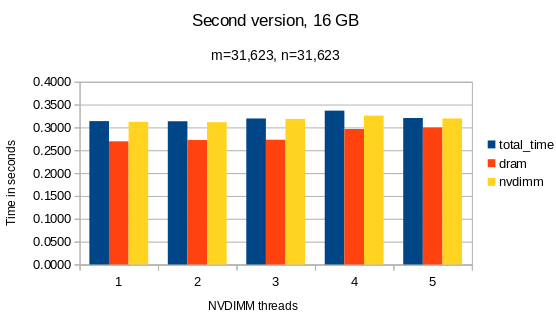
\includegraphics[scale=0.7]{Large_Array_test/Second_version_16GB.png}
\caption{Result of the second version of the code with 16 GB of data in graph form.}
\label{fig:SecondVersion16GB}
\end{figure}

When comparing the predicted DRAM time in table \ref{tab:Prediction16GB} to the measured DRAM time in table \ref{tab:SecondVersion16GB} one can see that at most the prediction is off by between 0.01 and 0.05 seconds.
The prediction DRAM time in table \ref{tab:Prediction160GB} is also quite accurate when compared to DRAM times measured in table \ref{tab:SecondVersion160GB}. The actual result is slower than the predicted time by between 0.2 and 0.5 seconds depending on how many threads have been given to NVIDMM.

The measured time of the NVDIMM in table \ref{tab:SecondVersion16GB} is slower than the predicted time in table \ref{tab:Prediction16GB}. The NVDIMM result is about 0.06 second slower than the predicted result, in percent it is around 20\% slower. 
The NVIDMM result in table \ref{tab:SecondVersion160GB} is also slower than the predicted NVDIMM time in \ref{tab:Prediction160GB}. All the NVDIMM times are between 1 and 2.5 second slower, in percent it would be between 23\% and 37\%.

All the total times in table \ref{tab:SecondVersion16GB} are also almost identical to the NVDIMM time. This version of the code all threads will update the ghost arrays when all of them are done with the their task so it was expected that the total time was a little slower than the NVDIMM time. The ghost arrays might be so small that they do not have any significant impact on the time.

The total time in table \ref{tab:SecondVersion160GB} is also slower than the NVDIMM time. This is because of the same reasons as mentions in last paragraph. The lowest difference between NVDIMM and total time is when just one thread is delegated and the difference is 0.11 seconds. The size of the ghost arrays does not change even though the amount of data on the NVDIMM increases, the length of the ghost arrays is always 100,000 elements. Because of this the difference between total time and NVDIMM should be the same for all the total time. This is not the case, all the other differences are between 0.65 and 1.16 seconds. There is no clear reason for why the test takes that long.

\begin{table}[!hbtp]
\centering
\begin{tabular}{ |c|c|c|c|c|c|c|c| }
\hline
&  & NVDIMM & DRAM & NVDIMM & DRAM & NVDIMM & Total \\
M & N & rows & threads & threads & time & time & time \\
\hline
100000 & 100000 & 2371 & 15 & 1 & 4.1319 & 4.8735 & 4.9889 \\
\hline
100000 & 100000 & 4724 & 14 & 2 & 4.0864 & 5.0859 & 6.0841 \\
\hline
100000 & 100000 & 7321 & 13 & 3 & 4.0079 & 5.5318 & 6.6954 \\
\hline
100000 & 100000 & 9885 & 12 & 4 & 4.1450 & 5.7829 & 6.5336 \\
\hline
100000 & 100000 & 12071 & 11 & 5 & 4.3569 & 6.0666 & 6.7233 \\
\hline
\end{tabular}
\caption{Result of the second version of the code with 160 GB of data.}
\label{tab:SecondVersion160GB}
\end{table}
\begin{figure}[!hbtp]
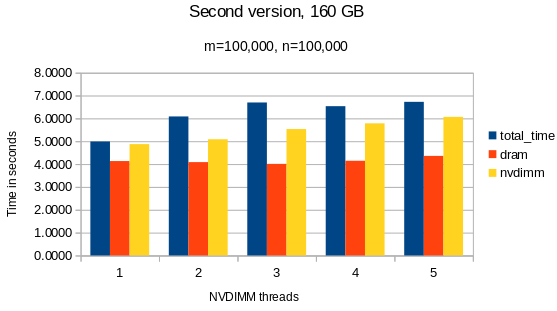
\includegraphics[scale=0.7]{Large_Array_test/Second_version_160GB.png}
\caption{Result of the second version of the code with 160 GB of data in graph form.}
\end{figure}

%\clearpage
\subsubsection{Comparisons of versions}
When comparing the two versions its possible to make a couple of observations. 
First in the 16 GB test the second version NVDIMM time and total time is faster in all instances and the DRAM in second version is faster three out of five times. The first version of DRAM time barely beat the second version of the test two times. 

In the 160 GB version of the test all the total time in the second version are faster then the first version. Three NVDIMM times and one DRAM time in the second version are faster then the first version.

Since there is no updating of the ghost array in the first version it should be faster then the second version, but this is not the case. In both the 16 GB and the 160 GB version the second version have a faster total time then the first version. If the total time in the first version were equal to NVDIMM which it should theoretically be then first version would have been faster then the second version in two instances. 

Based on the result in the first and second version, the extra work of updating the ghost array does not make the second version slower then the first version. The code in the second version is also more readable then the first version because it does not have all of the it-sentences and code that repeats itself. 

Overall the second version is the better version based on the total time and the readability of the code. 




%%%%%%%%%%%%%%%%%%%%%%%%%%%%%%%%%%%%%%%%%%%%%%%%%%%%%%%%%%%%%%%%%%%%%%%
%			Kommentert ut skrift									  %
%%%%%%%%%%%%%%%%%%%%%%%%%%%%%%%%%%%%%%%%%%%%%%%%%%%%%%%%%%%%%%%%%%%%%%%

\begin{comment}
Column six shows the average speed of all the DRAM threads in the test. The test is repeated ten times so if eleven DRAM threads then there are 99 DRAM threads that will be taken average of. The first test is excluded because the times are way higher then all the tests that comes after. 
The two next column is the dram minimum and dram maximum. Dram minimum is found by first finding the fastest DRAM thread in each of the nine tests and then take the average of them. 
Dram maximum is calculated the same way as dram minimum, The only difference is that this is for the slowest speed. 
Column nine, ten and eleven shows nvdimm average, nvdimm minimum and nvdimm maximum. These column are similar to dram average, dram minimum and dram maximum. The different is that the times is for the nvdimm threads.
The last three column is the total average, total minimum and total maximum. The total time is only measured once for each test so total minimum and total maximum shows the fastest and slowest test. Total average is the average of all the tests except the first test. 
\end{comment}

\begin{comment}
\begin{figure}[!hbtp]
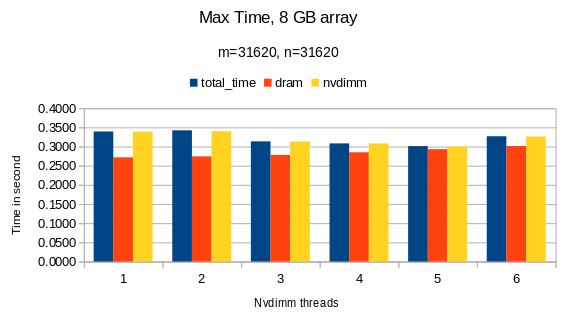
\includegraphics[scale=0.7]{Large_Array_test/FirstVersion_MaxTime_8GB_array.png}
\caption{First version, max time}
\end{figure}

\begin{figure}[!hbtp]
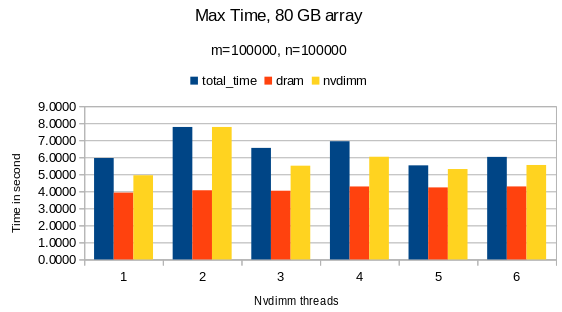
\includegraphics[scale=0.7]{Large_Array_test/FirstVersion_MaxTime_80GB_array.png}
\caption{First version, max time}
\end{figure}
\begin{figure}[!hbtp]
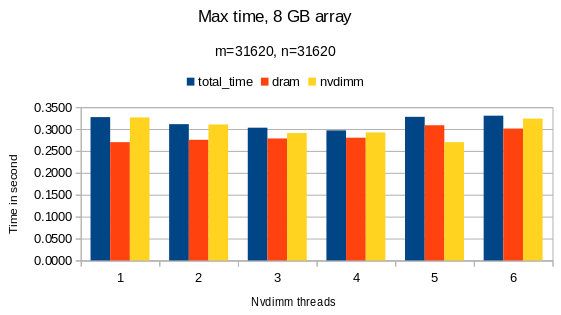
\includegraphics[scale=0.7]{Large_Array_test/SecondVersion_MaxTime_8GB_array.png}
\caption{second version, max time}
\end{figure}

\begin{figure}[!hbtp]
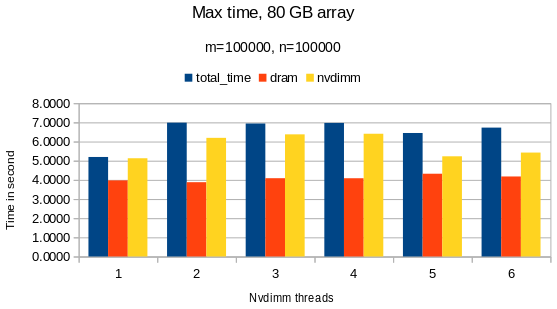
\includegraphics[scale=0.7]{Large_Array_test/SecondVersion_MaxTime_80GB_array.png}
\caption{second version, max time}
\end{figure}

\begin{table}[!hbtp]
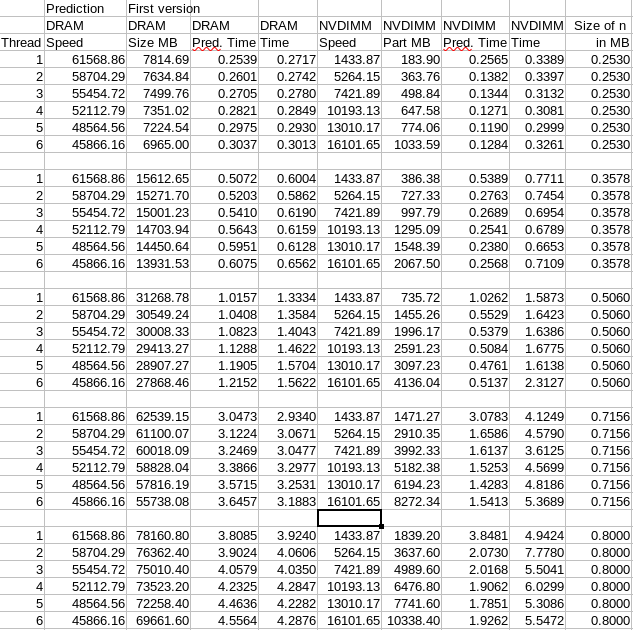
\includegraphics[scale=0.6]{Large_Array_test/FirstVersion_Prediction.png}
\caption{First version, Prediction}
\end{table}
\begin{table}[!hbtp]
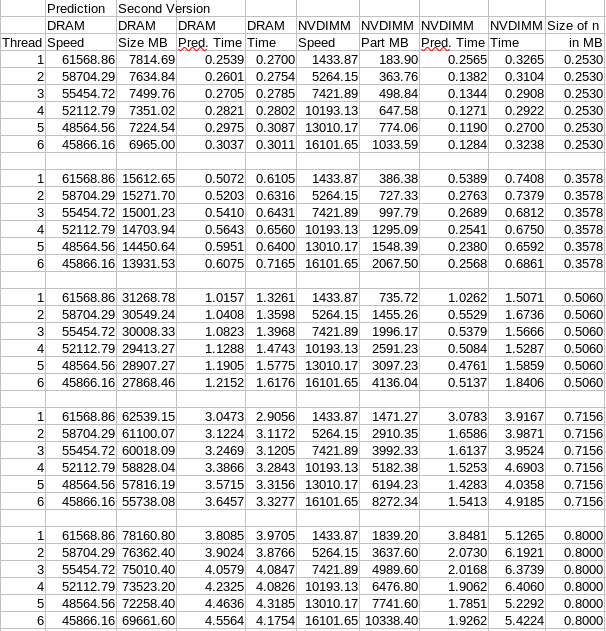
\includegraphics[scale=0.6]{Large_Array_test/SecondVersion_Prediction.png}
\caption{Second version, Prediction}
\end{table}


\begin{table}[!hbtp]
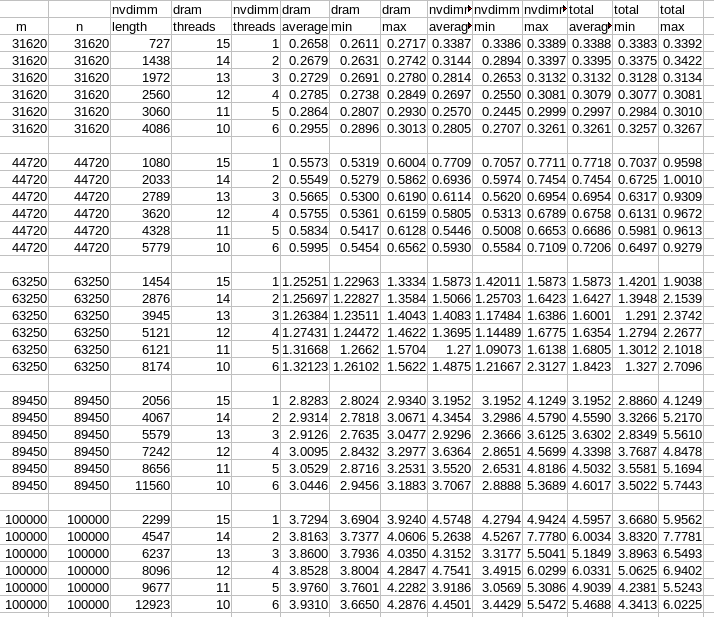
\includegraphics[scale=0.6]{Large_Array_test/FirstVersion_MaxTime_Table.png}
\caption{First version, result}
\end{table}
\begin{table}[!hbtp]
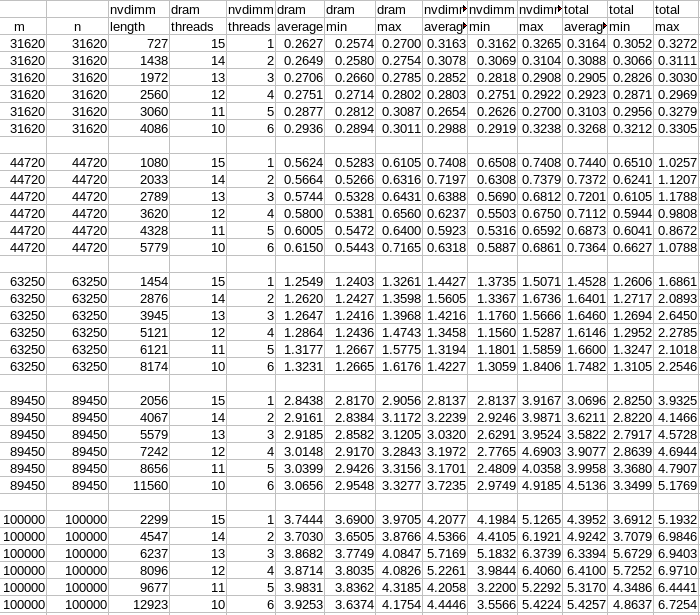
\includegraphics[scale=0.6]{Large_Array_test/SecondVersion_MaxTime_Table.png}
\caption{second version, result}
\end{table}
\end{comment}


\begin{comment}
FIRST VERSION

\begin{figure}[!hbtp]
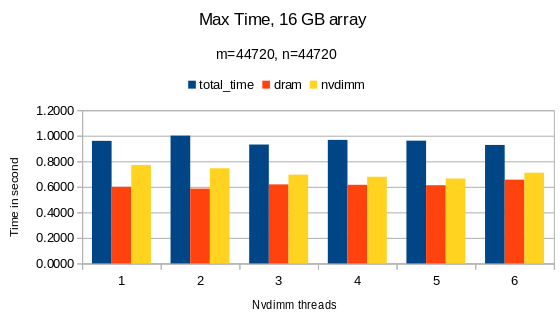
\includegraphics[scale=0.7]{Large_Array_test/FirstVersion_MaxTime_16GB_array.png}
\caption{First version, max time}
\end{figure}
\begin{figure}[!hbtp]
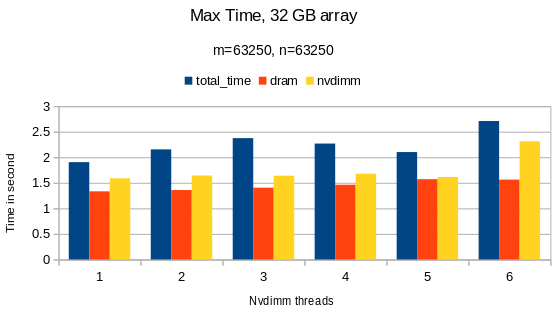
\includegraphics[scale=0.7]{Large_Array_test/FirstVersion_MaxTime_32GB_array.png}
\caption{First version, max time}
\end{figure}
\begin{figure}[!hbtp]
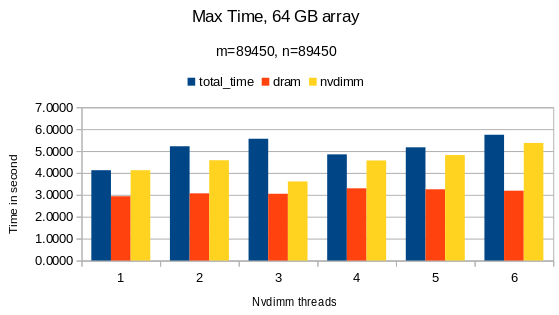
\includegraphics[scale=0.7]{Large_Array_test/FirstVersion_MaxTime_64GB_array.png}
\caption{First version, max time}
\end{figure}

%\begin{comment}
\begin{table}
\begin{tabular}{ |c|c|c|c|c|c| }
\hline
Nvdimm & Dram & Nvdimm & Dram & Nvdimm & Total \\
length & threads & threads & time & time & time \\
\hline
2399 & 15 & 1 & 4.172096 & 5.817548 & 5.817570 \\
\hline
4753 & 14 & 2 & 3.911470 & 6.300235 & 6.715596 \\
\hline
7294 & 13 & 3 & 3.923727 & 6.821659 & 7.982469 \\
\hline
9752 & 12 & 4 & 3.944112 & 7.032991 & 8.281379 \\
\hline
12290 & 11 & 5 & 3.967966 & 6.668957 & 7.374679 \\
\hline
14790 & 10 & 6 & 4.056013 & 6.795332 & 7.927536 \\
\hline
\end{tabular}
\caption{First version, result}
\end{table}
%\end{comment}
\begin{figure}[!hbtp]
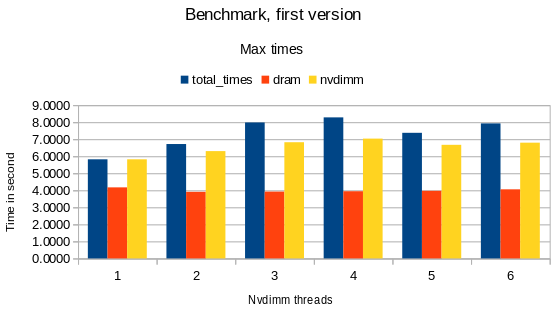
\includegraphics[scale=0.7]{Large_Array_test/First_version_100k_100k_MaxTime.png}
\caption{First version, max time}
\end{figure}

\clearpage
\subsubsection{Raw data}
\begin{table}[!hbtp]
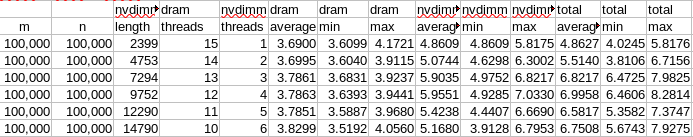
\includegraphics[scale=0.6]{Large_Array_test/First_version_100k_100k_Table.png}
\caption{First version, result}
\end{table}

\begin{table}[!hbtp]
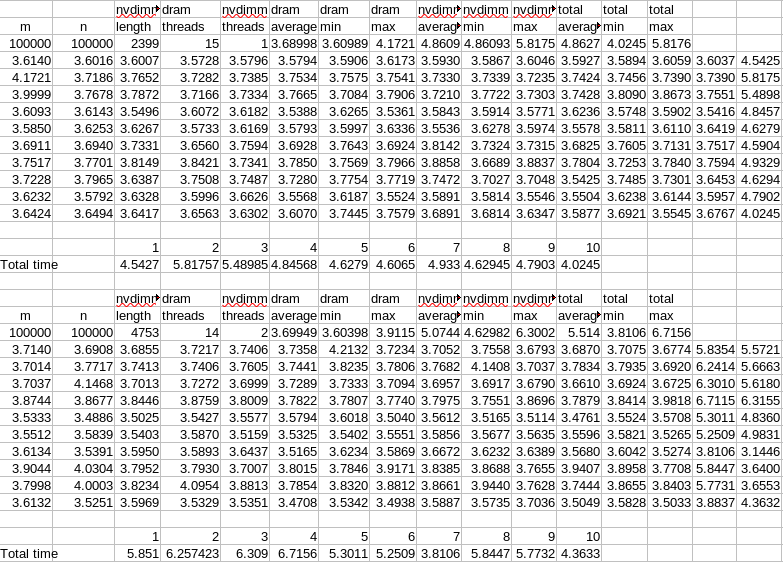
\includegraphics[scale=0.6]{Large_Array_test/First_version_100k_100k_Raw_1.png}
\caption{First version, result}
\end{table}
\begin{table}[!hbtp]
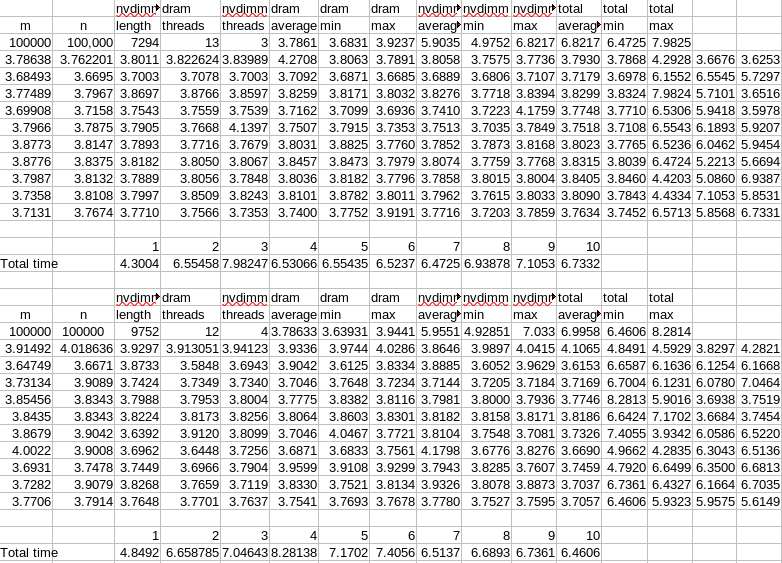
\includegraphics[scale=0.6]{Large_Array_test/First_version_100k_100k_Raw_2.png}
\caption{First version, result}
\end{table}
\begin{table}[!hbtp]
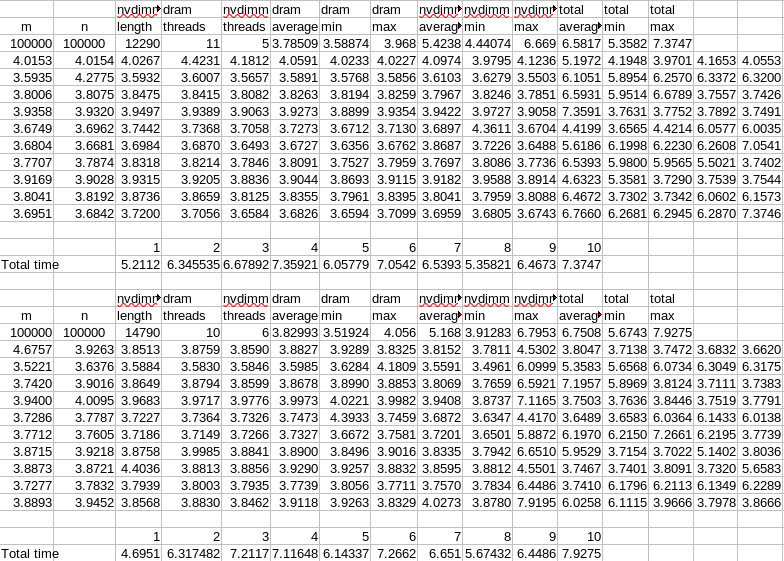
\includegraphics[scale=0.6]{Large_Array_test/First_version_100k_100k_Raw_3.png}
\caption{First version, result}
\end{table}

\clearpage
\subsubsection{From previous weeks}

\begin{table}[!hbtp]
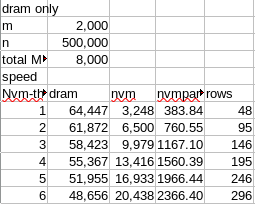
\includegraphics[scale=0.6]{Large_Array_test/First_version_2k_500k_Distibution.png}
\caption{First version, distribution}
\end{table}

\begin{table}[!hbtp]
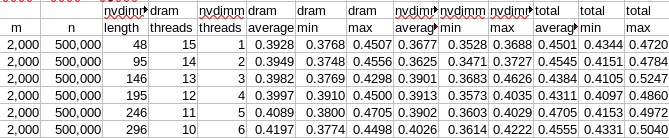
\includegraphics[scale=0.6]{Large_Array_test/First_version_2k_500k_Table.png}
\caption{First version, result}
\end{table}

\begin{figure}[!hbtp]
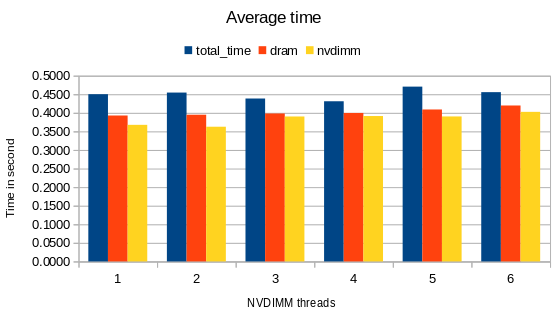
\includegraphics[scale=0.7]{Large_Array_test/First_version_2k_500k_average.png}
\caption{First version, max time}
\end{figure}

\begin{figure}[!hbtp]
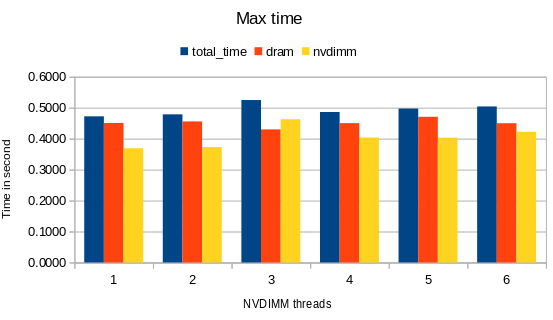
\includegraphics[scale=0.7]{Large_Array_test/First_version_2k_500k_MaxTime.png}
\caption{First version, minimum time}
\end{figure}

\begin{figure}[!hbtp]
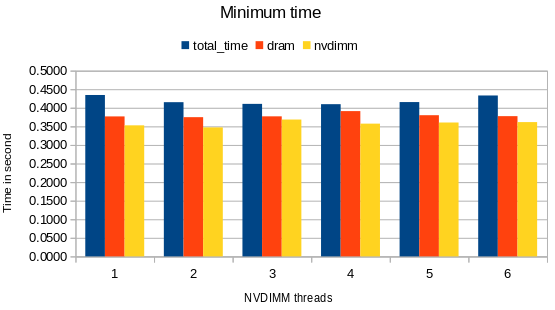
\includegraphics[scale=0.7]{Large_Array_test/First_version_2k_500k_MinTime.png}
\caption{First version, average time}
\end{figure}

\clearpage
Where N is 1'000'000
\begin{table}[!hbtp]
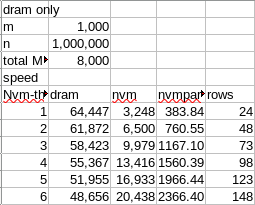
\includegraphics[scale=0.6]{Large_Array_test/First_version_1k_1000k_Distribution.png}
\caption{First version, distribution}
\end{table}

\begin{table}[!hbtp]
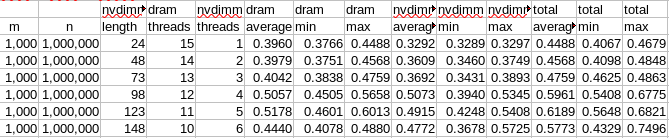
\includegraphics[scale=0.6]{Large_Array_test/First_version_1k_1000k_Table.png}
\caption{First version, result}
\end{table}

\begin{figure}[!hbtp]
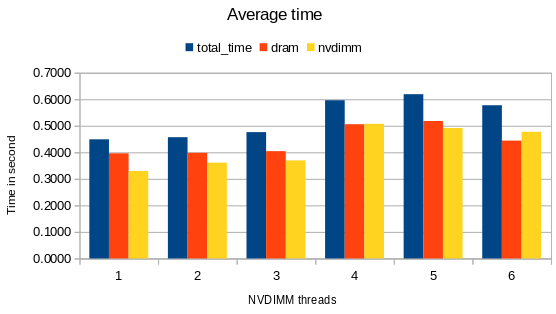
\includegraphics[scale=0.7]{Large_Array_test/First_version_1k_1000k_average.png}
\caption{First version, max time}
\end{figure}

\begin{figure}[!hbtp]
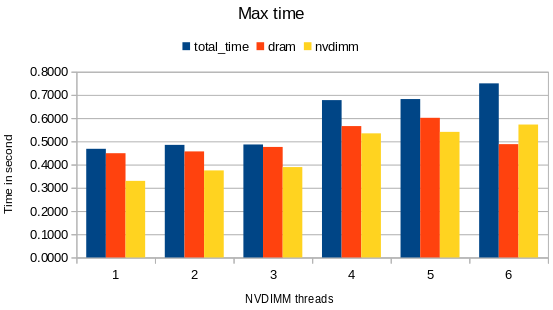
\includegraphics[scale=0.7]{Large_Array_test/First_version_1k_1000k_MaxTime.png}
\caption{First version, minimum time}
\end{figure}

\begin{figure}[!hbtp]
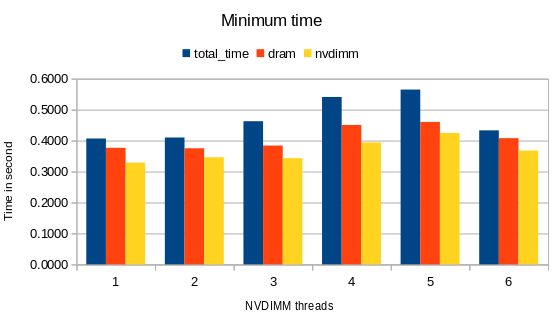
\includegraphics[scale=0.7]{Large_Array_test/First_version_1k_1000k_MinTime.png}
\caption{First version, average time}
\end{figure}

\begin{table}[!hbtp]
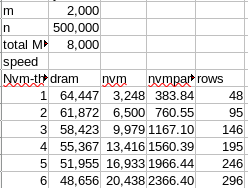
\includegraphics[scale=0.6]{Large_Array_test/Large_Array_test_fordeling.png}
\caption{First version, distribution}
\end{table}

\begin{table}[!hbtp]
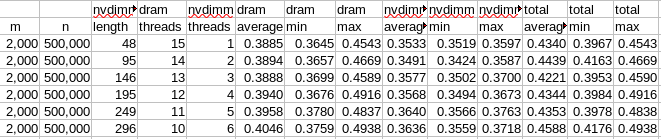
\includegraphics[scale=0.6]{Large_Array_test/First_version_v3_table.png}
\caption{First version, result}
\end{table}

\begin{figure}[!hbtp]
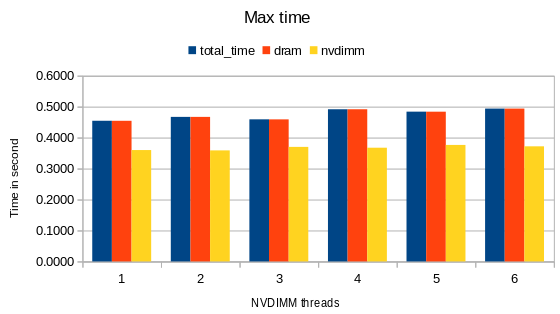
\includegraphics[scale=0.7]{Large_Array_test/First_version_v3_figur_1.png}
\caption{First version, max time}
\end{figure}

\begin{figure}[!hbtp]
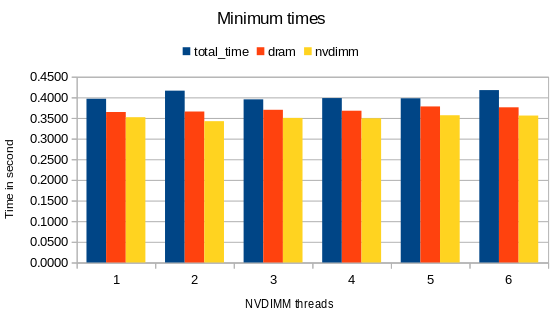
\includegraphics[scale=0.7]{Large_Array_test/First_version_v3_figur_2.png}
\caption{First version, minimum time}
\end{figure}

\begin{figure}[!hbtp]
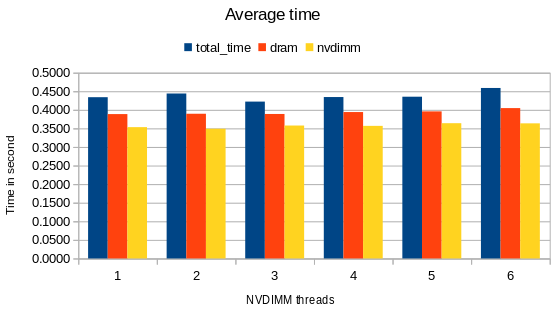
\includegraphics[scale=0.7]{Large_Array_test/First_version_v3_figur_3.png}
\caption{First version, average time}
\end{figure}

%---------------------

\begin{table}[!hbtp]
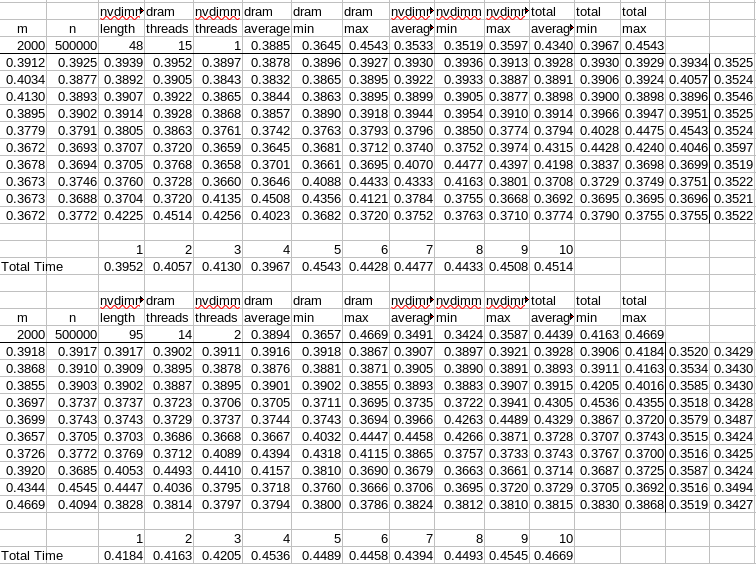
\includegraphics[scale=0.6]{Large_Array_test/Large_array_test_first_version_v3_part1.png}
\caption{First version part 1}
\end{table}

\begin{table}[!hbtp]
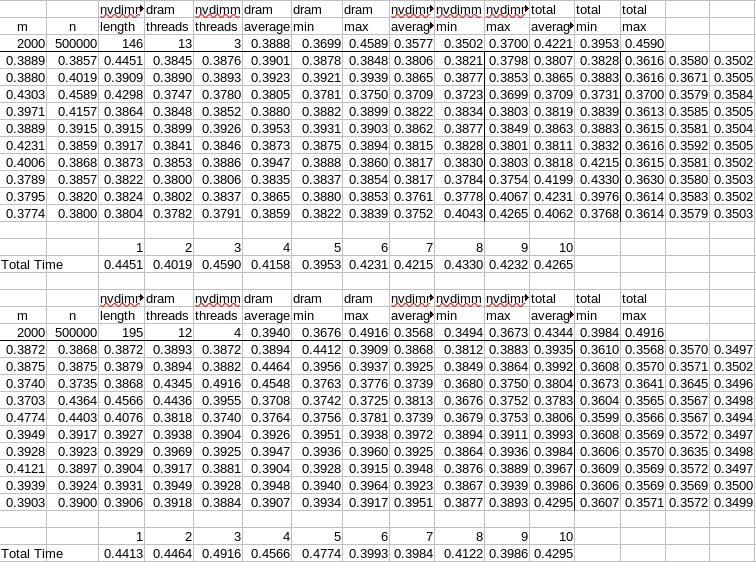
\includegraphics[scale=0.6]{Large_Array_test/Large_array_test_first_version_v3_part2.png}
\caption{First version part 2}
\end{table}

\begin{table}[!hbtp]
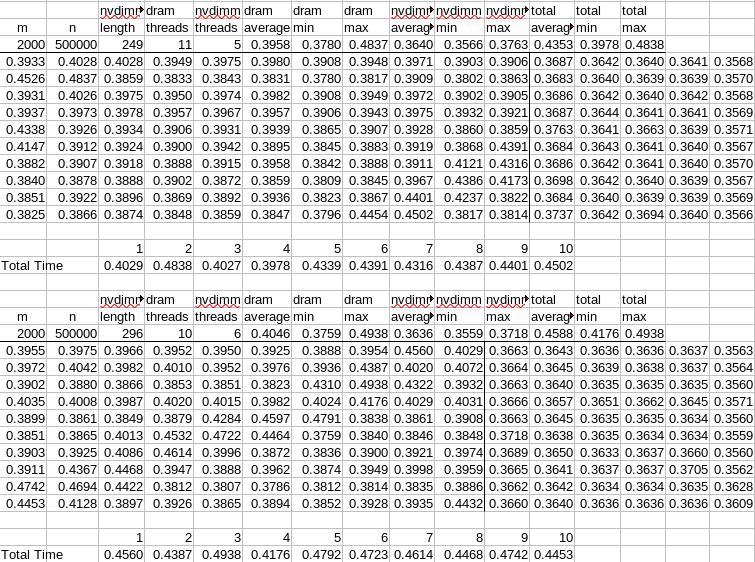
\includegraphics[scale=0.6]{Large_Array_test/Large_array_test_first_version_v3_part3.png}
\caption{First version part 3}
\end{table}

\begin{table}[!hbtp]
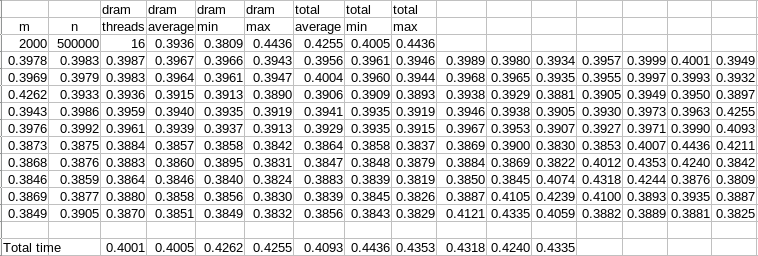
\includegraphics[scale=0.6]{Large_Array_test/Large_array_test_first_version_DRAM_only.png}
\caption{First version, dram only}
\end{table}

\end{comment}

\begin{comment}
SECOND VERSION

\begin{figure}[!hbtp]
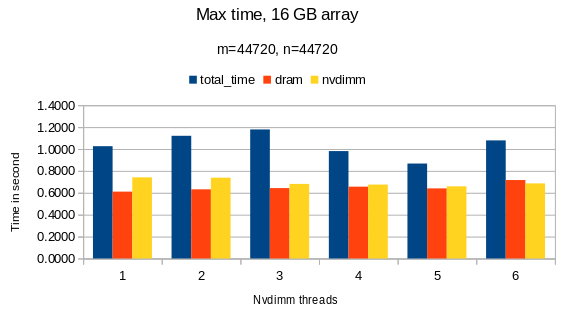
\includegraphics[scale=0.7]{Large_Array_test/SecondVersion_MaxTime_16GB_array.png}
\caption{second version, max time}
\end{figure}
\begin{figure}[!hbtp]
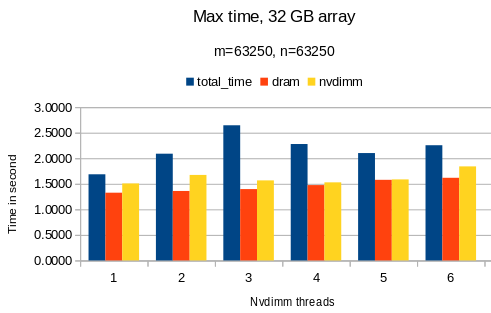
\includegraphics[scale=0.7]{Large_Array_test/SecondVersion_MaxTime_32GB_array.png}
\caption{second version, max time}
\end{figure}
\begin{figure}[!hbtp]
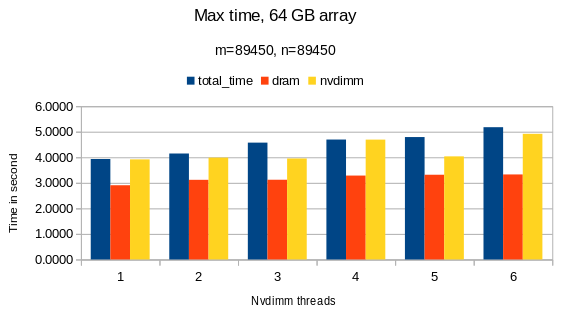
\includegraphics[scale=0.7]{Large_Array_test/SecondVersion_MaxTime_64GB_array.png}
\caption{second version, max time}
\end{figure}

\begin{table}[!hbtp]
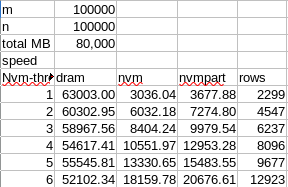
\includegraphics[scale=0.6]{Large_Array_test/First_version_100k_100k_Distibution_v2.png}
\caption{Second version, distribution}
\end{table}
\begin{table}
\begin{tabular}{ |c|c|c|c|c|c| }
\hline
Nvdimm & Dram & Nvdimm & Dram & Nvdimm & Total \\
length & threads & threads & time & time & time \\
\hline
 2399 & 15 & 1 & 3.871935 & 5.551327 & 5.551754 \\
\hline
 4753 & 14 & 2 & 3.833448 & 6.311746 & 7.576095 \\
\hline
 7294 & 13 & 3 & 3.984483 & 7.278315 & 8.031769 \\
\hline
 9752 & 12 & 4 & 3.907516 & 7.348314 & 8.072969 \\
\hline
 12290 & 11 & 5 & 3.947991 & 7.241239 & 8.072641 \\
\hline
 14790 & 10 & 6 & 3.800333 & 7.463296 & 8.262591 \\
\hline
\end{tabular}
\caption{Second version, result}
\end{table}

\begin{figure}[!hbtp]
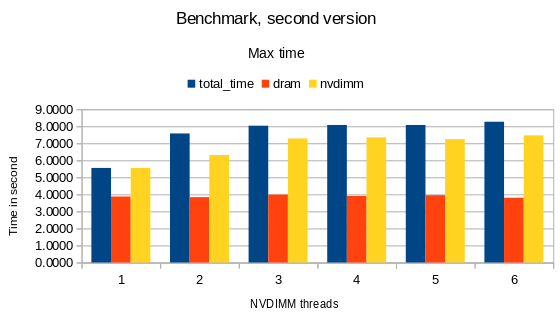
\includegraphics[scale=0.7]{Large_Array_test/Second_version_100k_100k_MaxTime.png}
\caption{Second version, max time}
\end{figure}



\clearpage
\subsubsection{Raw data}

\begin{table}[!hbtp]
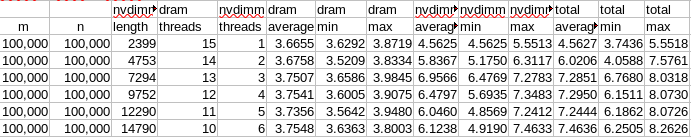
\includegraphics[scale=0.6]{Large_Array_test/Second_version_100k_100k_Table.png}
\caption{Second version, result}
\end{table}

\begin{table}[!hbtp]
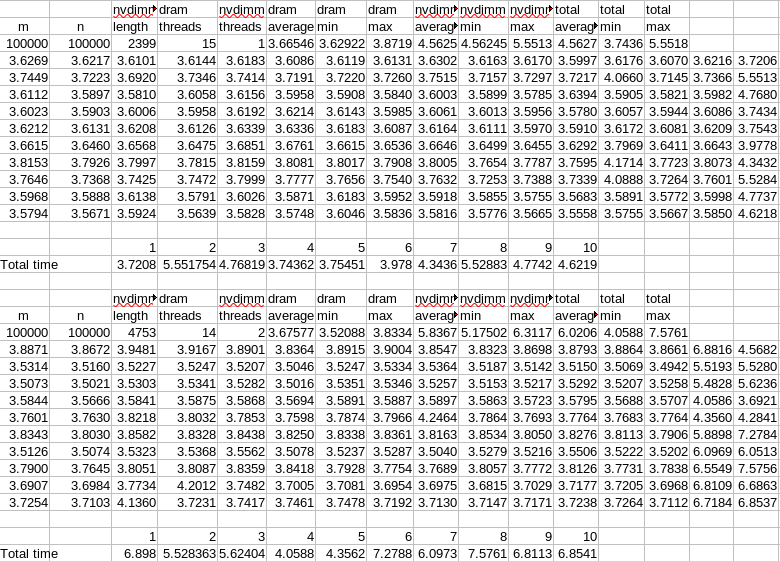
\includegraphics[scale=0.6]{Large_Array_test/Second_version_100k_100k_Raw_1.png}
\caption{Second version, result}
\end{table}
\begin{table}[!hbtp]
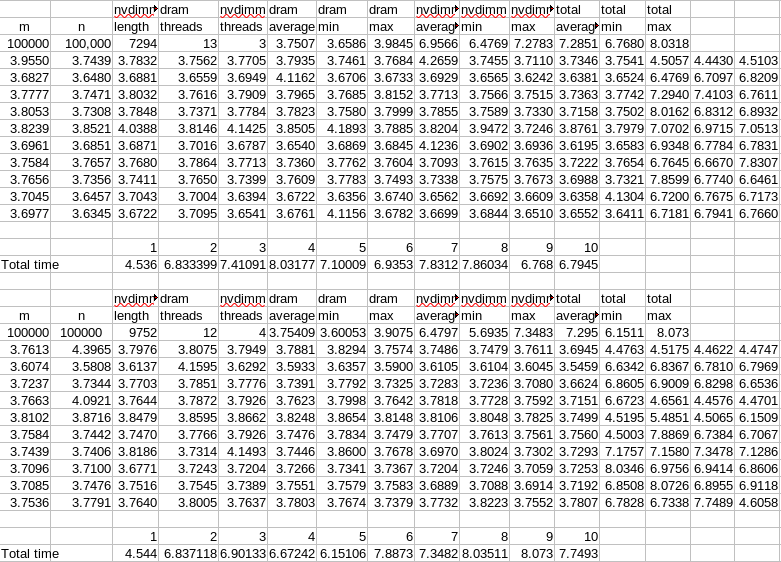
\includegraphics[scale=0.6]{Large_Array_test/Second_version_100k_100k_Raw_2.png}
\caption{Second version, result}
\end{table}
\begin{table}[!hbtp]
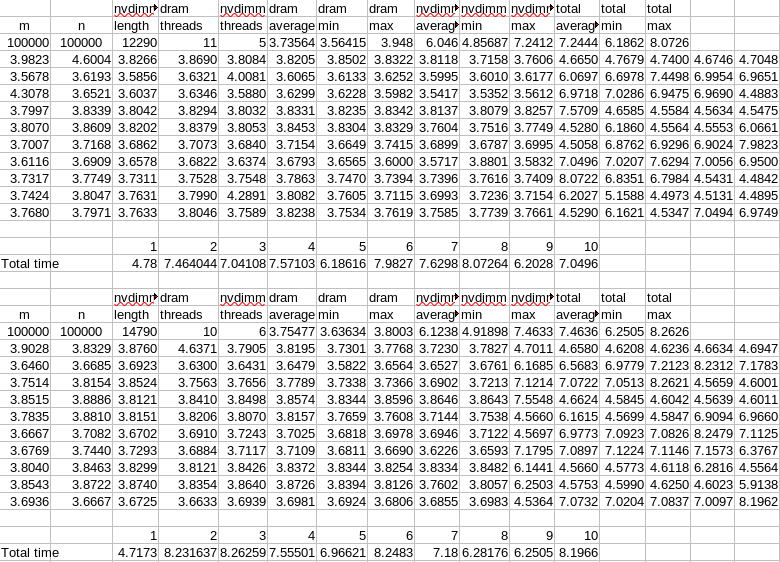
\includegraphics[scale=0.6]{Large_Array_test/Second_version_100k_100k_Raw_3.png}
\caption{Second version, result}
\end{table}

\clearpage
\subsection{From previous weeks}
\begin{table}[!hbtp]
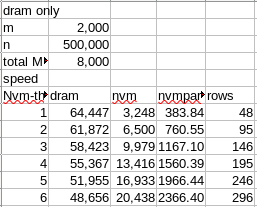
\includegraphics[scale=0.6]{Large_Array_test/Second_version_2k_500k_Distribution.png}
\caption{Second version, distribution}
\end{table}

\begin{table}[!hbtp]
\includegraphics[scale=0.6]{Large_Array_test/Second_version_2k_500k_Table.png}
\caption{Second version, result}
\end{table}

\begin{figure}[!hbtp]
\includegraphics[scale=0.7]{Large_Array_test/Second_version_2k_500k_Average.png}
\caption{Second version, max time}
\end{figure}

\begin{figure}[!hbtp]
\includegraphics[scale=0.7]{Large_Array_test/Second_version_2k_500k_MaxTime.png}
\caption{Second version, minimum time}
\end{figure}

\begin{figure}[!hbtp]
\includegraphics[scale=0.7]{Large_Array_test/Second_version_2k_500k_MinTime.png}
\caption{Second version, average time}
\end{figure}

\begin{table}[!hbtp]
\includegraphics[scale=0.6]{Large_Array_test/Second_version_2k_500000_raw_1.png}
\caption{Second version part 1}
\end{table}

\begin{table}[!hbtp]
\includegraphics[scale=0.6]{Large_Array_test/Second_version_2k_500000_raw_2.png}
\caption{Second version part 2}
\end{table}

\begin{table}[!hbtp]
\includegraphics[scale=0.6]{Large_Array_test/Second_version_2k_500000_raw_3.png}
\caption{Second version part 3}
\end{table}

\clearpage
Where N is 1'000'000
\begin{table}[!hbtp]
\includegraphics[scale=0.6]{Large_Array_test/Second_version_1k_1000k_Distribution.png}
\caption{Second version, distribution}
\end{table}

\begin{table}[!hbtp]
\includegraphics[scale=0.6]{Large_Array_test/Second_version_1k_1000k_Table.png}
\caption{Second version, result}
\end{table}

\begin{figure}[!hbtp]
\includegraphics[scale=0.7]{Large_Array_test/Second_version_1k_1000k_average.png}
\caption{Second version, max time}
\end{figure}

\begin{figure}[!hbtp]
\includegraphics[scale=0.7]{Large_Array_test/Second_version_1k_1000k_MaxTime.png}
\caption{Second version, minimum time}
\end{figure}

\begin{figure}[!hbtp]
\includegraphics[scale=0.7]{Large_Array_test/Second_version_1k_1000k_MinTime.png}
\caption{Second version, average time}
\end{figure}

\begin{table}[!hbtp]
\includegraphics[scale=0.6]{Large_Array_test/Large_Array_test_fordeling.png}
\caption{First version, distribution}
\end{table}

\begin{table}[!hbtp]
\includegraphics[scale=0.6]{Large_Array_test/Large_array_test_second_version_v3_part1.png}
\caption{First version part 1}
\end{table}

\begin{table}[!hbtp]
\includegraphics[scale=0.6]{Large_Array_test/Large_array_test_second_version_v3_part2.png}
\caption{First version part 2}
\end{table}

\begin{table}[!hbtp]
\includegraphics[scale=0.6]{Large_Array_test/Large_array_test_second_version_v3_part3.png}
\caption{First version part 3}
\end{table}

\begin{table}[!hbtp]
\includegraphics[scale=0.6]{First_version_DRAM_only_17_9_21.png}
\caption{First version, dram only}
\end{table}

\begin{table}[!hbtp]
\includegraphics[scale=0.6]{first_version_more_detailed_1.png}
\caption{First version, more detailed 1}
\end{table}

\begin{table}[!hbtp]
\includegraphics[scale=0.6]{first_version_more_detailed_2.png}
\caption{First version, more detailed 2.}
\end{table}

\begin{table}[!hbtp]
\includegraphics[scale=0.7]{Large_array_test_first_version_v5.png}
\caption{First version.}
\end{table}

\begin{table}[!hbtp]
\includegraphics[scale=0.7]{Large_array_test_second_version_v3.png}
\caption{Second version.}
\end{table}

\begin{table}[!hbtp]
\includegraphics[scale=0.7]{Large_array_test_first_version_v2.png}
\caption{First version. OLD}
\end{table}

\begin{table}[!hbtp]
\includegraphics[scale=0.7]{Large_array_test_first_version_v3.png}
\caption{First version. OLD}
\end{table}

\begin{table}[!hbtp]
\includegraphics[scale=0.7]{Large_array_test_second_version_v2.png}
\caption{Second version. OLD}
\end{table}

\begin{table}[!hbtp]
\includegraphics[scale=0.7]{Large_array_test_second_version_NVDIMM_only_v2.png}
\caption{NVDIMM only of second version. OLD}
\end{table}

\begin{table}[!hbtp]
\includegraphics[scale=0.7]{DRAM_only_on_n50.png}
\caption{DRAM only on n50. OLD}
\end{table}

\end{comment}

\end{document}               % End of document.
